\documentclass[../Thesis-IJspeert.tex]{subfiles}

\begin{document}

\graphicspath{ {"Hologram Generation with Spatial Light Modulators/figs/"} }
\pgfplotsset{table/search path={"Hologram Generation with Spatial Light Modulators/data/"}}

\chapter{Hologram Generation with Spatial Light Modulators}
\addtocontents{toc}{\vskip-6pt\par\noindent\protect\textcolor{gray75}{\protect\rule{\textwidth}{0.5pt}}\par}orizontal line to ToC
\label{chap:HologramGenerationwithSpatialLightModulators}

\section{Introduction}
blablba

\section{Algorithms for hologram generation}
As shown in \autoref{setup}, we use a liquid crystal SLM with an active area of $\SI{7.68}{\milli\meter} \times\SI{7.68}{\milli\meter}$ to imprint a specific phase profile (kinoform) on the incident beam in order to generate the desired diffraction pattern in the trapping plane. Although analytic kinoform solutions exist for certain target intensity profiles \cite{Matsumoto2008,Moulder2012}, finding the optimal phase pattern is a non-trivial problem that often requires a numerical approach. The difficulty results from the incomplete a priori knowledge of the light field in both planes. Whilst the intensity is constrained to the target pattern in the trapping plane, the phase is not. Similarly, in the holographic plane at the SLM interface, the intensity is constrained to the Gaussian profile of the incident light, which leaves the phase as a variable to be optimised. Many iterative phase retrieval methods are based on an iterative Fourier transform algorithm (IFTA). These include the Gerchberg-Saxton (GS) algorithm \cite{GS} and many of its modifications: weighted-GS (GSW) \cite{DiLeonardo2007}, mixed-region amplitude freedom (MRAF) \cite{Pasienski2008}, offset-MRAF (OMRAF) \cite{Gaunt2012} and softness-OMRAF (SOMRAF) \cite{somraf}. Alternative methods include the Floyd-Steinberg error diffusion dithering algorithm \cite{floyd} and conjugate gradient minimisation \cite{Harte2014}. In the following sections, we outline the principles of GSW, MRAF and conjugate gradient minimisation, followed by a discussion on the performance of these algorithms in the context of generating optical potentials for single atom traps.

\subsection{Gerchberg-Saxton}

\subsection{Mixed-region amplitude freedom}
A frequently employed method for the generation of holographic optical tweezers is the MRAF algorithm, which is schematically shown in \autoref{fig:mraf}.
\begin{figure}[h]
	\centering
	\begin{tikzpicture}
	\node[anchor=south west,inner sep=0] (image) at (0,0) {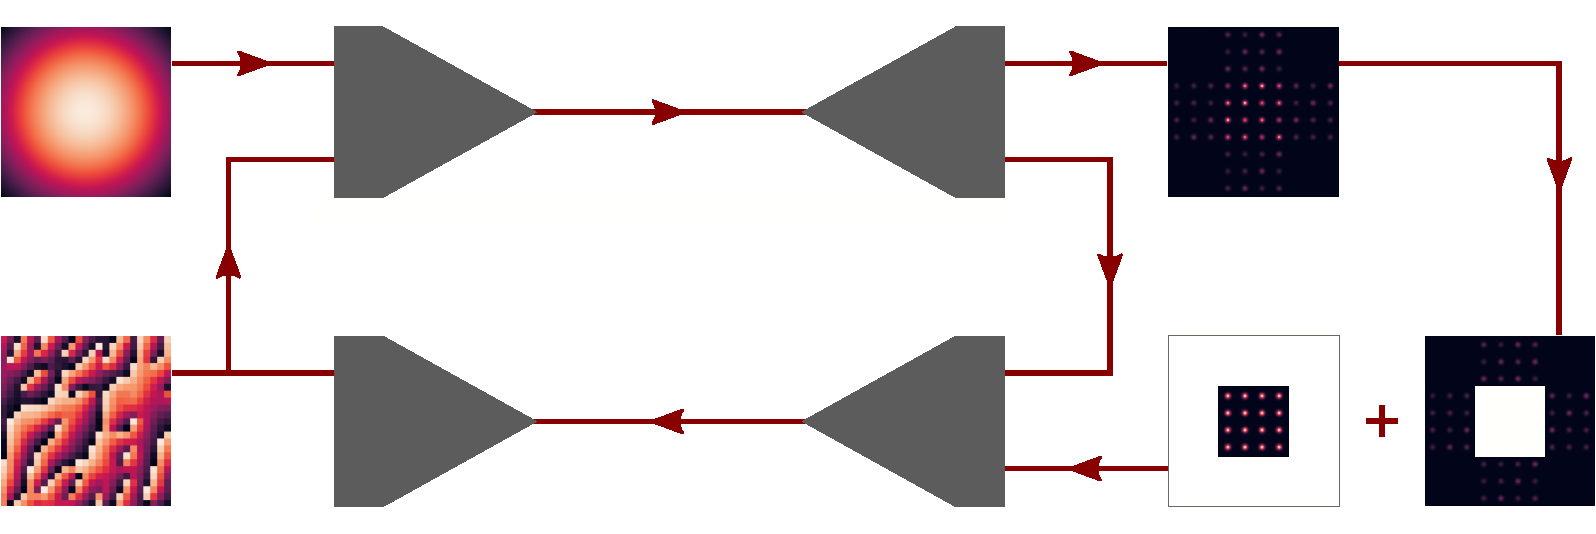
\includegraphics[width=0.85\textwidth]{MRAF.pdf}};
	\begin{scope}[x={(image.south east)},y={(image.north west)}]
	
	%\draw[help lines,xstep=.1,ystep=.1] (0,0) grid (1,1);
	%\foreach \x in {0,1,...,9} { \node [anchor=north] at (\x/10,0) {0.\x}; }
	%\foreach \y in {0,1,...,9} { \node [anchor=east] at (0,\y/10) {0.\y}; }
	
	\node[] at (0.235,0.71) {\small\textcolor{white}{$\phi$}};
	\node[] at (0.235,0.86) {\small\textcolor{white}{$I$}};
	
	\node[] at (0.605,0.71) {\small\textcolor{white}{$\phi$}};
	\node[] at (0.605,0.86) {\small\textcolor{white}{$I$}};
	
	\node[] at (0.235,0.135) {\small\textcolor{white}{$I$}};
	\node[] at (0.235,0.285) {\small\textcolor{white}{$\phi$}};
	
	\node[] at (0.605,0.135) {\small\textcolor{white}{$I$}};
	\node[] at (0.605,0.285) {\small\textcolor{white}{$\phi$}};
	
	\node[align=center] at (0.42,0.89) {\small\textcolor{markrood}{$\mathcal{F}$}};
	\node[align=center] at (0.43,0.33) {\small\textcolor{markrood}{$\mathcal{F}^{-1}$}};
	
	\node[rectangle, rounded corners=1mm, minimum size=5mm, text width=25mm,
	anchor=base, very thick, draw=none, fill=none, align=right] at (0.01,0.5) {\small\textcolor{markgrijs}{Intensity}};
	
	\node[rectangle, rounded corners=1mm, minimum size=5mm, text width=25mm,
	anchor=base, very thick, draw=none, fill=none, align=right] at (0.05,-0.08) {\small\textcolor{markgrijs}{Phase pattern}};
	
	\node[rectangle, rounded corners=1mm, minimum size=5mm, text width=30mm,
	anchor=base, very thick, draw=none, fill=none, align=left] at (0.85,0.5) {\small\textcolor{markgrijs}{Approximation}};
	
	\node[rectangle, rounded corners=1mm, minimum size=5mm, text width=25mm,
	anchor=base, very thick, draw=none, fill=none, align=left] at (0.844,-0.08) {\small\textcolor{markgrijs}{Target}};
	
	\node[rectangle, rounded corners=1mm, minimum size=5mm, text width=25mm,
	anchor=base, very thick, draw=none, fill=none, align=left] at (0.985,-0.08) {\small\textcolor{markgrijs}{Periphery}};
	
	\end{scope}
	
	
	\end{tikzpicture}
	\caption[An example of a floating figure]{Diagram of the iterative mixed-region amplitude freedom algorithm used for calculating the phase pattern in the holographic plane (left hand side) that corresponds to the target intensity profile in the trapping plane (right hand side).} % The text in the square bracket is the caption for the list of figures while the text in the curly brackets is the figure caption
	\label{fig:mraf} 
\end{figure}
The MRAF algorithm provides a good trade-off between accuracy and speed. For generating large grids, it is more accurate than error diffusion dithering \cite{Holland2018}. 

In addition, we have measured that MRAF is faster than conjugate gradient minimisation by a factor of at least $20$. In the first iteration, the algorithm computes the 2D Fourier transform of the incident intensity profile combined with an initial phase guess, which yields an approximate solution for the diffracted light in the trapping plane. The algorithm then extracts the phase from this image and recombines it with an intensity profile that consists of the target intensity in the region of interest and the approximated intensity outside this region (periphery). This gives the algorithm more freedom to converge with respect to the conventional GS algorithm. The final step consists of an inverse transformation from which the kinoform is extracted and recombined with the incident intensity profile prior to starting the next iteration. The algorithm is terminated if the difference between the target and approximation is sufficiently small or if the maximum number of iteration is reached.

\section{Algorithm benchmarking}

\subsection{Gerchberg-Saxton based algorithms}

\subsubsection{Simulated trap intensity and homogeneity}

\begin{figure}[t]
	\vspace{0em}
\hspace{-0.4em}
\begin{tikzpicture}
\begin{groupplot}[group style={group size=4 by 2,horizontal sep=0.65cm, vertical sep=0.65cm},height=4cm,width=4cm,no markers]
\nextgroupplot
[
width=4cm,
enlargelimits=false,
axis on top,    % <-- (use with `matrix plot*')
colormap/viridis,
point meta=explicit,
% change me to adjust ``end point'' values used for the colormap
point meta min=0.045,
point meta max=0.085,
xticklabels={,,},
% change min and max values to just show that interval in the colorbar
%            colorbar style={
%                ymin=0.5e7,
%                ymax=2.5e7,
%            },
]
%            \addplot [matrix plot] table [meta=funceval] {
\addplot [matrix plot*] table [meta expr=\thisrowno{2}] {grid_GS.csv};
\nextgroupplot
[
width=4cm,
enlargelimits=false,
axis on top,    % <-- (use with `matrix plot*')
colormap/viridis,
point meta=explicit,
% change me to adjust ``end point'' values used for the colormap
point meta min=0.045,
point meta max=0.085,
xticklabels={,,},
yticklabels={,,}
% change min and max values to just show that interval in the colorbar
%            colorbar style={
%                ymin=0.5e7,
%                ymax=2.5e7,
%            },
]
%            \addplot [matrix plot] table [meta=funceval] {
\addplot [matrix plot*] table [meta expr=\thisrowno{2}] {grid_MRAF80.csv};

\nextgroupplot
[
width=4cm,
enlargelimits=false,
axis on top,    % <-- (use with `matrix plot*')
colormap/viridis,
point meta=explicit,
% change me to adjust ``end point'' values used for the colormap
point meta min=0.045,
point meta max=0.085,
xticklabels={,,},
yticklabels={,,}
% change min and max values to just show that interval in the colorbar
%            colorbar style={
%                ymin=0.5e7,
%                ymax=2.5e7,
%            },
]
%            \addplot [matrix plot] table [meta=funceval] {
            \addplot [matrix plot*] table [meta expr=\thisrowno{2}] {grid_MRAF90.csv};
         
\nextgroupplot
[
width=4cm,
enlargelimits=false,
axis on top,    % <-- (use with `matrix plot*')
colormap/viridis,
colorbar,
point meta=explicit,
% change me to adjust ``end point'' values used for the colormap
point meta min=0.045,
point meta max=0.085,
xticklabels={,,},
yticklabels={,,}
% change min and max values to just show that interval in the colorbar
%            colorbar style={
%                ymin=0.5e7,
%                ymax=2.5e7,
%            },
]
%            \addplot [matrix plot] table [meta=funceval] {
\addplot [matrix plot*] table [meta expr=\thisrowno{2}] {grid_MRAF99.csv};

\nextgroupplot
[
ylabel={\hspace{8em}$y$},
width=4cm,
enlargelimits=false,
axis on top,    % <-- (use with `matrix plot*')
colormap/viridis,
point meta=explicit,
% change me to adjust ``end point'' values used for the colormap
point meta min=0.045,
point meta max=0.085,
% change min and max values to just show that interval in the colorbar
%            colorbar style={
%                ymin=0.5e7,
%                ymax=2.5e7,
%            },
]
%            \addplot [matrix plot] table [meta=funceval] {
\addplot [matrix plot*] table [meta expr=\thisrowno{2}] {grid_AD.csv};

\nextgroupplot
[
xlabel={\hspace{8em}$x$},
width=4cm,
enlargelimits=false,
axis on top,    % <-- (use with `matrix plot*')
colormap/viridis,
point meta=explicit,
% change me to adjust ``end point'' values used for the colormap
point meta min=0.045,
point meta max=0.085,
yticklabels={,,}
% change min and max values to just show that interval in the colorbar
%            colorbar style={
%                ymin=0.5e7,
%                ymax=2.5e7,
%            },
]
%            \addplot [matrix plot] table [meta=funceval] {
\addplot [matrix plot*] table [meta expr=\thisrowno{2}] {grid_ADMRAF80.csv};

\nextgroupplot
[
width=4cm,
enlargelimits=false,
axis on top,    % <-- (use with `matrix plot*')
colormap/viridis,
point meta=explicit,
% change me to adjust ``end point'' values used for the colormap
point meta min=0.045,
point meta max=0.085,
yticklabels={,,}
% change min and max values to just show that interval in the colorbar
%            colorbar style={
%                ymin=0.5e7,
%                ymax=2.5e7,
%            },
]
%            \addplot [matrix plot] table [meta=funceval] {
\addplot [matrix plot*] table [meta expr=\thisrowno{2}] {grid_ADMRAF90.csv};

\nextgroupplot
[
width=4cm,
enlargelimits=false,
axis on top,    % <-- (use with `matrix plot*')
colormap/viridis,
colorbar,
point meta=explicit,
% change me to adjust ``end point'' values used for the colormap
point meta min=0.045,
point meta max=0.085,
yticklabels={,,}
% change min and max values to just show that interval in the colorbar
%            colorbar style={
%                ymin=0.5e7,
%                ymax=2.5e7,
%            },
]
%            \addplot [matrix plot] table [meta=funceval] {
\addplot [matrix plot*] table [meta expr=\thisrowno{2}] {grid_ADMRAF99.csv};

\end{groupplot}
\end{tikzpicture}
	\caption{(a) Recorded light intensity in the trapping plane. (b) Corresponding grid of optical power per trap in mW. (c) Integrated atom fluorescence. The box marks the 5 traps used for analysis of the ac-Stark shift (see \autoref{stark}). The $1/e^2$ diameter of the traps is $2.2\,\mu$m.}
\end{figure}

\begin{figure}[t]
	\vspace{0em}
	\centering
	\begin{subfigure}[b]{.23\linewidth}
		\begin{tikzpicture}
		\centering
		\node[inner sep=0] (image) {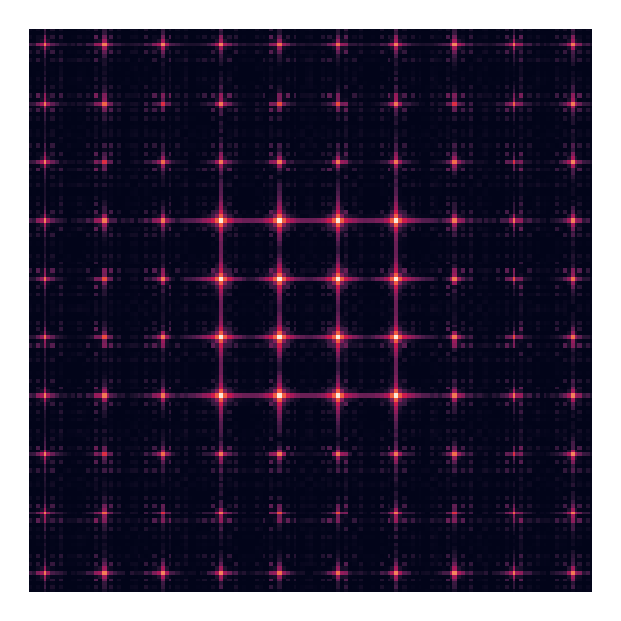
\includegraphics[width=3cm] {approxint_GS.pdf}};;
		\end{tikzpicture}
		\centering
		\caption{}
		\label{a}
	\end{subfigure}
	\begin{subfigure}[b]{.23\linewidth}
		\begin{tikzpicture}
		\centering
		\node[inner sep=0] (image) {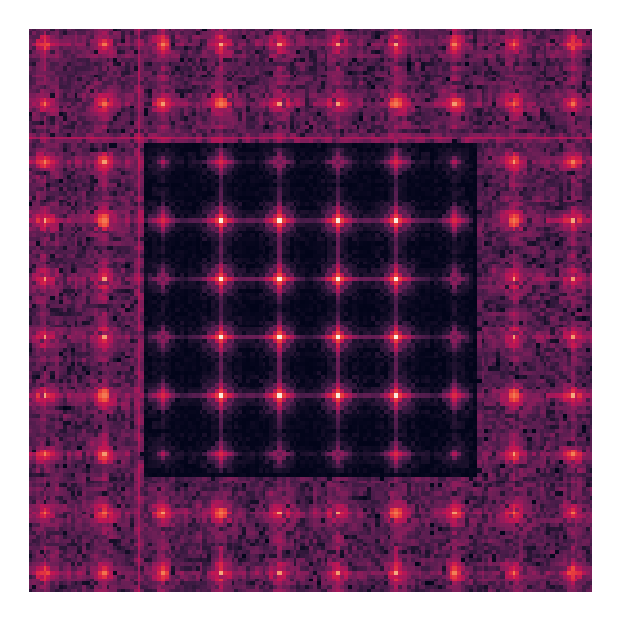
\includegraphics[width=3cm] {approxint_MRAF80.pdf}};;
		\end{tikzpicture}
		\centering
		\caption{}
		\label{b}
	\end{subfigure}
	\begin{subfigure}[b]{.23\linewidth}
		\begin{tikzpicture}
		\centering
		\node[inner sep=0] (image) {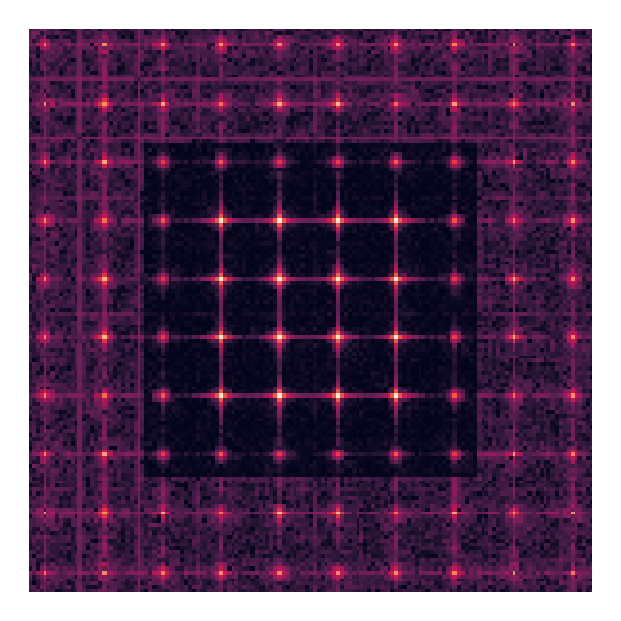
\includegraphics[width=3cm] {approxint_MRAF90.pdf}};;
		\end{tikzpicture}
		\centering
		\caption{}
		\label{c}
	\end{subfigure}
	\begin{subfigure}[b]{.23\linewidth}
		\begin{tikzpicture}
		\centering
		\node[inner sep=0] (image) {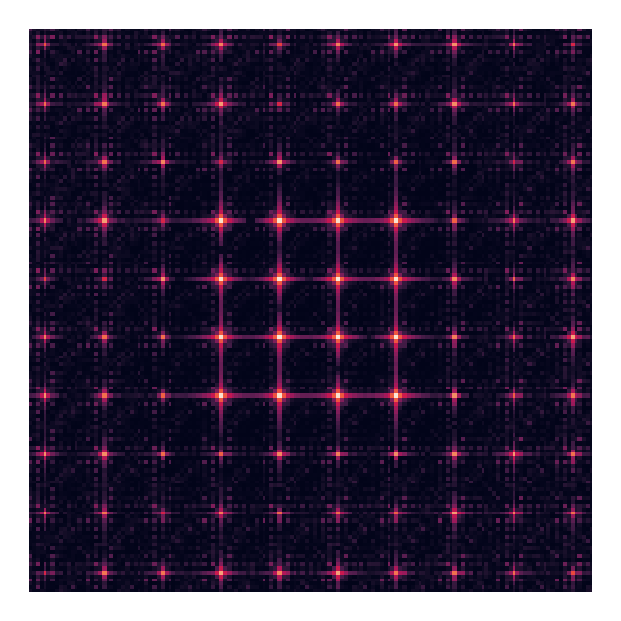
\includegraphics[width=3cm] {approxint_MRAF99.pdf}};;
		\end{tikzpicture}
		\centering
		\caption{}
		\label{c}
	\end{subfigure}
\\
\vspace{0.2em}
	\begin{subfigure}[b]{.23\linewidth}
	\begin{tikzpicture}
	\centering
	\node[inner sep=0] (image) {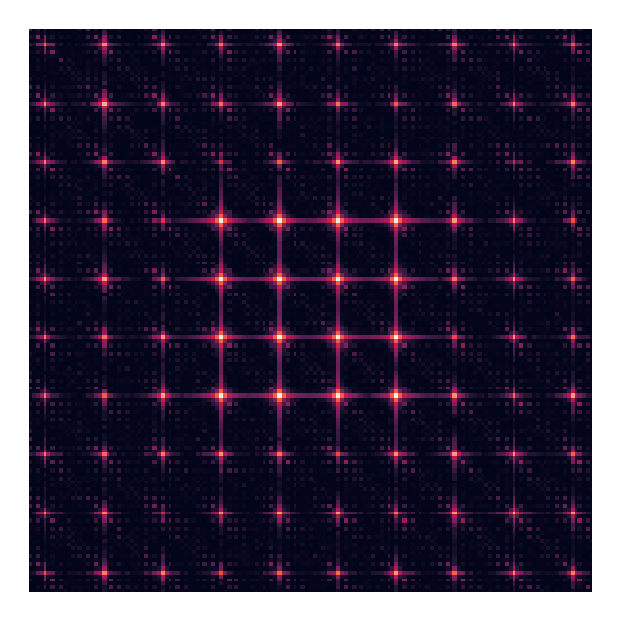
\includegraphics[width=3cm] {approxint_AD.pdf}};;
	\end{tikzpicture}
	\centering
	\caption{}
	\label{a}
\end{subfigure}
\begin{subfigure}[b]{.23\linewidth}
	\begin{tikzpicture}
	\centering
	\node[inner sep=0] (image) {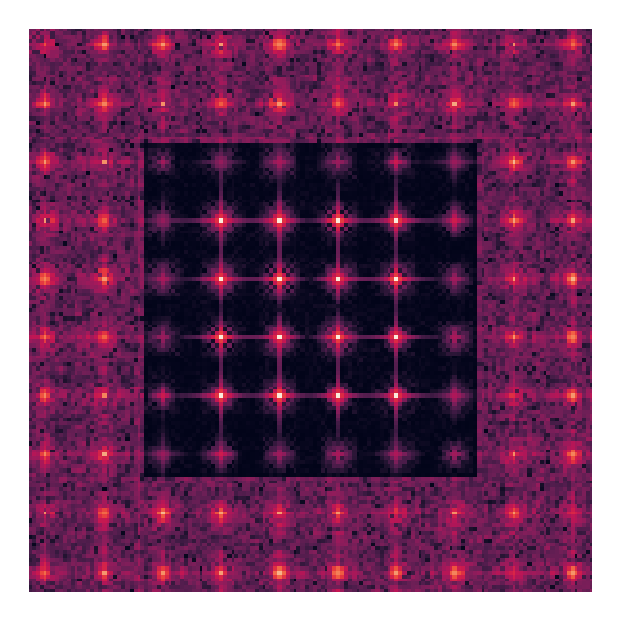
\includegraphics[width=3cm] {approxint_ADMRAF80.pdf}};;
	\end{tikzpicture}
	\centering
	\caption{}
	\label{b}
\end{subfigure}
\begin{subfigure}[b]{.23\linewidth}
	\begin{tikzpicture}
	\centering
	\node[inner sep=0] (image) {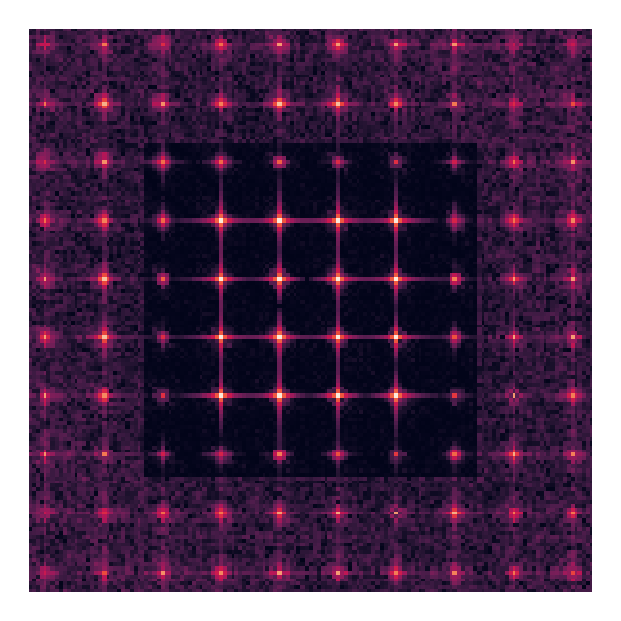
\includegraphics[width=3cm] {approxint_ADMRAF90.pdf}};;
	\end{tikzpicture}
	\centering
	\caption{}
	\label{c}
\end{subfigure}
\begin{subfigure}[b]{.23\linewidth}
	\begin{tikzpicture}
	\centering
	\node[inner sep=0] (image) {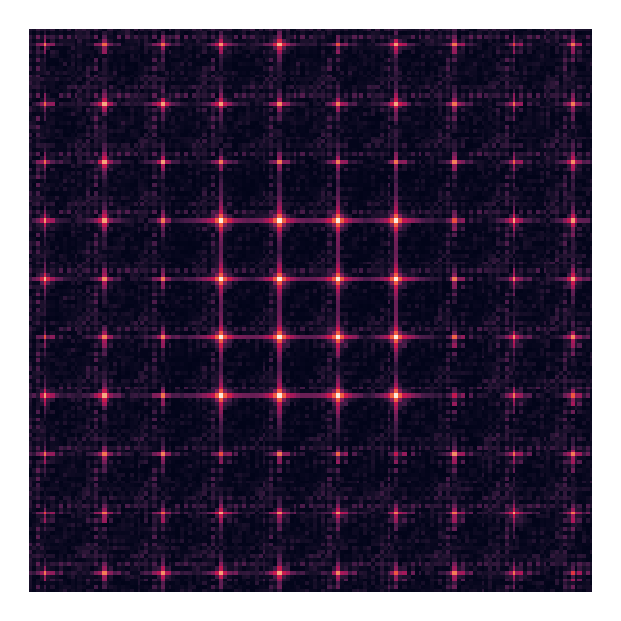
\includegraphics[width=3cm] {approxint_ADMRAF99.pdf}};;
	\end{tikzpicture}
	\centering
	\caption{}
	\label{c}
\end{subfigure}
	\caption{(a) what is plotted is the log(10e-9 plus intensity)Recorded light intensity in the trapping plane. (b) Corresponding grid of optical power per trap in mW. (c) Integrated atom fluorescence. The box marks the 5 traps used for analysis of the ac-Stark shift (see \autoref{stark}). The $1/e^2$ diameter of the traps is $2.2\,\mu$m.}
\end{figure}


\begin{figure}[t]
	%\vspace{0.7em}
	\centering
	\begin{tikzpicture}
	
	\begin{groupplot}[group style={group size=4 by 2,horizontal sep=0.65cm, vertical sep=0.65cm},height=4cm,width=4cm,no markers]
	\nextgroupplot
	[
	xmin=10, xmax=75,
	ymin=-0.005, ymax=0.085,
	%xtick={0,20,40,60,80,100},
	%ytick={0,20,40,60,80,100,120},
	%legend pos=north west,
	ymajorgrids=true,
	xmajorgrids=true,
	grid style=dashed,
	xticklabels={,,},
	]
	
	\addplot[
	color=markrood,
	] table [x index = 0, y index = 1]{crosssection_targetint0_GS.csv};
	
	\addplot[
	only marks,
	mark = *,
	color=markdiepblauw,
	mark size=0.8pt
	] table [x index = 0, y index = 1]{crosssection_approxint_GS.csv};
	
	\nextgroupplot
	[
	xmin=10, xmax=75,
	ymin=-0.005, ymax=0.085,
	%xtick={0,20,40,60,80,100},
	%ytick={0,20,40,60,80,100,120},
	%legend pos=north west,
	ymajorgrids=true,
	xmajorgrids=true,
	grid style=dashed,
	xticklabels={,,},
	yticklabels={,,}
	]
	
	\addplot[
	color=markrood,
	] table [x index = 0, y index = 1]{crosssection_targetint0_MRAF80.csv};
	
	\addplot[
	only marks,
	mark = *,
	color=markdiepblauw,
	mark size=0.8pt
	] table [x index = 0, y index = 1]{crosssection_approxint_MRAF80.csv};
	
	\nextgroupplot
	[
	xmin=10, xmax=75,
	ymin=-0.005, ymax=0.085,
	%xtick={0,20,40,60,80,100},
	%ytick={0,20,40,60,80,100,120},
	%legend pos=north west,
	ymajorgrids=true,
	xmajorgrids=true,
	grid style=dashed,
	xticklabels={,,},
	yticklabels={,,}
	]
	
	\addplot[
	color=markrood,
	] table [x index = 0, y index = 1]{crosssection_targetint0_MRAF90.csv};
	
	\addplot[
	only marks,
	mark = *,
	color=markdiepblauw,
	mark size=0.8pt
	] table [x index = 0, y index = 1]{crosssection_approxint_MRAF90.csv};
	
	\nextgroupplot
	[
	xmin=10, xmax=75,
	ymin=-0.005, ymax=0.085,
	%xtick={0,20,40,60,80,100},
	%ytick={0,20,40,60,80,100,120},
	%legend pos=north west,
	ymajorgrids=true,
	xmajorgrids=true,
	grid style=dashed,
	xticklabels={,,},
	yticklabels={,,}
	]
	
	\addplot[
	color=markrood,
	] table [x index = 0, y index = 1]{crosssection_targetint0_MRAF99.csv};
	
	\addplot[
	only marks,
	mark = *,
	color=markdiepblauw,
	mark size=0.8pt
	] table [x index = 0, y index = 1]{crosssection_approxint_MRAF99.csv};
	
	\nextgroupplot
	[
	%xlabel={Pixel number},
	ylabel={\hspace{8em}$\sfrac{I}{I_\text{tot}}$},
	xmin=10, xmax=75,
	ymin=-0.005, ymax=0.085,
	%xtick={0,20,40,60,80,100},
	%ytick={0,20,40,60,80,100,120},
	%legend pos=north west,
	ymajorgrids=true,
	xmajorgrids=true,
	grid style=dashed,
	]
	
	\addplot[
	color=markrood,
	] table [x index = 0, y index = 1]{crosssection_targetint0_AD.csv};
	
	\addplot[
	only marks,
	mark = *,
	color=markdiepblauw,
	mark size=0.8pt
	] table [x index = 0, y index = 1]{crosssection_approxint_AD.csv};
	
	\nextgroupplot
	[
	xlabel={\hspace{8em}Pixel number},
	xmin=10, xmax=75,
	ymin=-0.005, ymax=0.085,
	%xtick={0,20,40,60,80,100},
	%ytick={0,20,40,60,80,100,120},
	%legend pos=north west,
	ymajorgrids=true,
	xmajorgrids=true,
	grid style=dashed,
	yticklabels={,,},
	]
	
	\addplot[
	color=markrood,
	] table [x index = 0, y index = 1]{crosssection_targetint0_ADMRAF80.csv};
	
	\addplot[
	only marks,
	mark = *,
	color=markdiepblauw,
	mark size=0.8pt
	] table [x index = 0, y index = 1]{crosssection_approxint_ADMRAF80.csv};
	
	\nextgroupplot
	[
	%xlabel={Pixel number},
	xmin=10, xmax=75,
	ymin=-0.005, ymax=0.085,
	%xtick={0,20,40,60,80,100},
	%ytick={0,20,40,60,80,100,120},
	%legend pos=north west,
	ymajorgrids=true,
	xmajorgrids=true,
	grid style=dashed,
	yticklabels={,,},
	]
	
	\addplot[
	color=markrood,
	] table [x index = 0, y index = 1]{crosssection_targetint0_ADMRAF90.csv};
	
	\addplot[
	only marks,
	mark = *,
	color=markdiepblauw,
	mark size=0.8pt
	] table [x index = 0, y index = 1]{crosssection_approxint_ADMRAF90.csv};
	
	\nextgroupplot
	[
	%xlabel={Pixel number},
	xmin=10, xmax=75,
	ymin=-0.005, ymax=0.085,
	%ymin=0, ymax=120,
	%xtick={0,20,40,60,80,100},
	%ytick={0,20,40,60,80,100,120},
	%legend pos=north west,
	ymajorgrids=true,
	xmajorgrids=true,
	grid style=dashed,
	yticklabels={,,},
	]
	
	\addplot[
	color=markrood,
	] table [x index = 0, y index = 1]{crosssection_targetint0_ADMRAF99.csv};
	
	\addplot[
	only marks,
	mark = *,
	color=markdiepblauw,
	mark size=0.8pt
	] table [x index = 0, y index = 1]{crosssection_approxint_ADMRAF99.csv};
	
	\end{groupplot}
	
	\end{tikzpicture}
	\caption[An example of a floating figure]{Average trap lifetime (left) and filling fraction (right) versus dipole trap power. Error bars represent the standard error of the mean based on up to three measurements of the fluorescence count rate ($50\,000$ frames) per trapping site.} % The text in the square bracket is the caption for the list of figures while the text in the curly brackets is the figure caption
	\label{fig:LTandFR} 
\end{figure}


\subsubsection{Measured trap intensity and homogeneity}


\begin{figure}[t]
	\vspace{0em}
	\centering
	\begin{subfigure}[b]{.23\linewidth}
		\begin{tikzpicture}
		\centering
		\node[inner sep=0] (image) {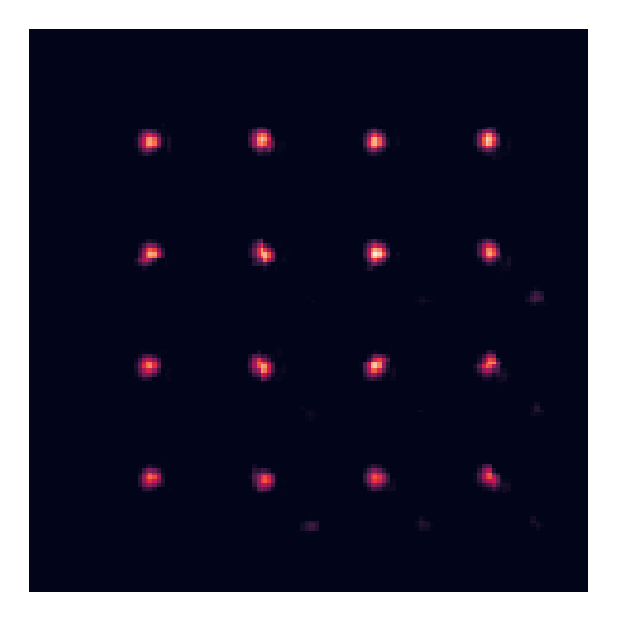
\includegraphics[width=3cm] {actualtraps_GS.pdf}};;
		\end{tikzpicture}
		\centering
		\caption{}
		\label{a}
	\end{subfigure}
	\begin{subfigure}[b]{.23\linewidth}
		\begin{tikzpicture}
		\centering
		\node[inner sep=0] (image) {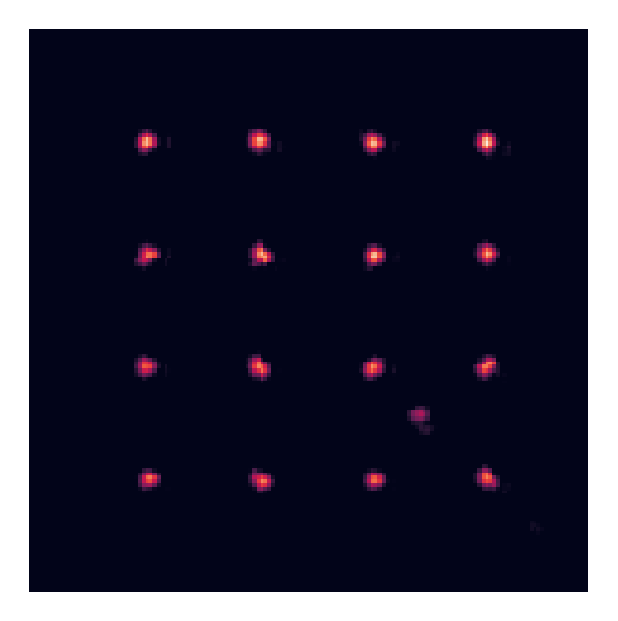
\includegraphics[width=3cm] {actualtraps_MRAF80.pdf}};;
		\end{tikzpicture}
		\centering
		\caption{}
		\label{b}
	\end{subfigure}
	\begin{subfigure}[b]{.23\linewidth}
		\begin{tikzpicture}
		\centering
		\node[inner sep=0] (image) {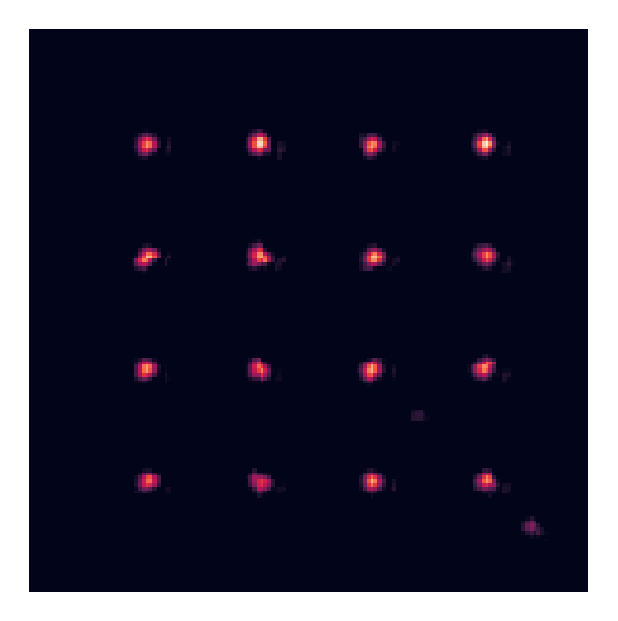
\includegraphics[width=3cm] {actualtraps_MRAF90.pdf}};;
		\end{tikzpicture}
		\centering
		\caption{}
		\label{c}
	\end{subfigure}
	\begin{subfigure}[b]{.23\linewidth}
		\begin{tikzpicture}
		\centering
		\node[inner sep=0] (image) {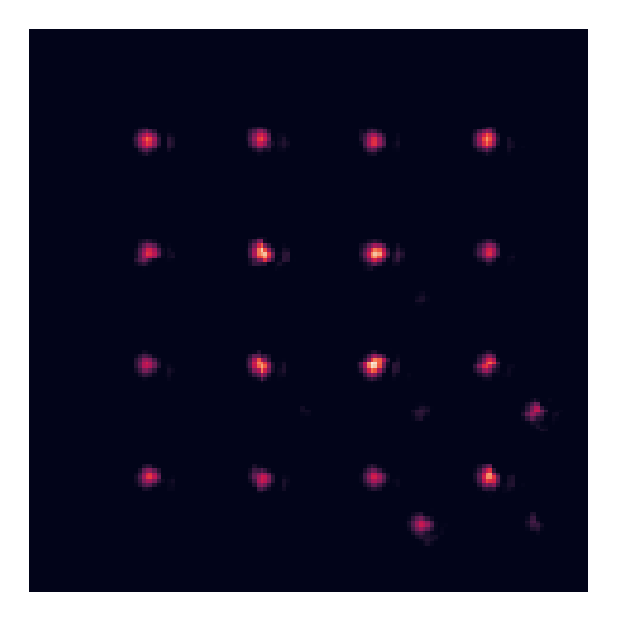
\includegraphics[width=3cm] {actualtraps_MRAF99.pdf}};;
		\end{tikzpicture}
		\centering
		\caption{}
		\label{c}
	\end{subfigure}
	\\
	\vspace{0.2em}
	\begin{subfigure}[b]{.23\linewidth}
		\begin{tikzpicture}
		\centering
		\node[inner sep=0] (image) {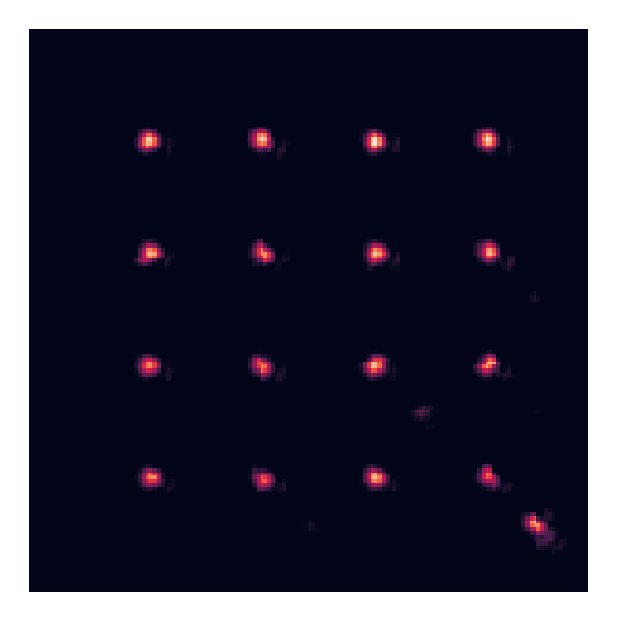
\includegraphics[width=3cm] {actualtraps_AD.pdf}};;
		\end{tikzpicture}
		\centering
		\caption{}
		\label{a}
	\end{subfigure}
	\begin{subfigure}[b]{.23\linewidth}
		\begin{tikzpicture}
		\centering
		\node[inner sep=0] (image) {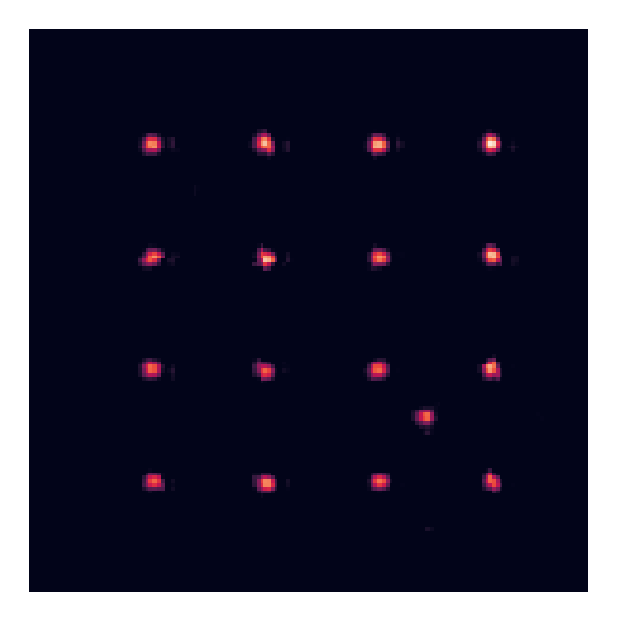
\includegraphics[width=3cm] {actualtraps_ADMRAF80.pdf}};;
		\end{tikzpicture}
		\centering
		\caption{}
		\label{b}
	\end{subfigure}
	\begin{subfigure}[b]{.23\linewidth}
		\begin{tikzpicture}
		\centering
		\node[inner sep=0] (image) {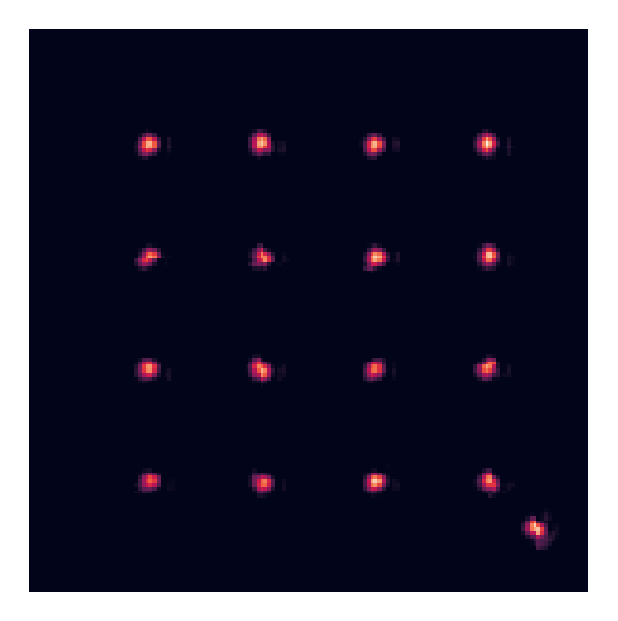
\includegraphics[width=3cm] {actualtraps_ADMRAF90.pdf}};;
		\end{tikzpicture}
		\centering
		\caption{}
		\label{c}
	\end{subfigure}
	\begin{subfigure}[b]{.23\linewidth}
		\begin{tikzpicture}
		\centering
		\node[inner sep=0] (image) {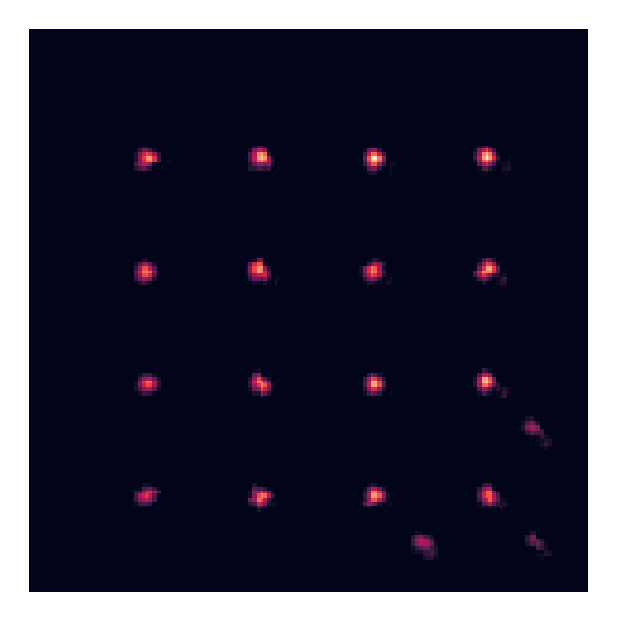
\includegraphics[width=3cm] {actualtraps_ADMRAF99.pdf}};;
		\end{tikzpicture}
		\centering
		\caption{}
		\label{c}
	\end{subfigure}
	\caption{(a) what is plotted is the log(10e-9 plus intensity)Recorded light intensity in the trapping plane. (b) Corresponding grid of optical power per trap in mW. (c) Integrated atom fluorescence. The box marks the 5 traps used for analysis of the ac-Stark shift (see \autoref{stark}). The $1/e^2$ diameter of the traps is $2.2\,\mu$m.}
\end{figure}

\begin{figure}[t]
	\vspace{0em}
	%\centering
	\hspace{-0.4em}
	\begin{tikzpicture}
	\begin{groupplot}[group style={group size=4 by 2,horizontal sep=0.65cm, vertical sep=0.65cm},height=4cm,width=4cm,no markers]
	\nextgroupplot
	[
	width=4cm,
	enlargelimits=false,
	axis on top,    % <-- (use with `matrix plot*')
	colormap/viridis,
	point meta=explicit,
	% change me to adjust ``end point'' values used for the colormap
	point meta min=0.01,
point meta max=0.05,
	xticklabels={,,},
	% change min and max values to just show that interval in the colorbar
	%            colorbar style={
	%                ymin=0.5e7,
	%                ymax=2.5e7,
	%            },
	]
	%            \addplot [matrix plot] table [meta=funceval] {
	\addplot [matrix plot*] table [meta expr=\thisrowno{2}] {measuredgrid_m_GS.csv};
	\nextgroupplot
	[
	width=4cm,
	enlargelimits=false,
	axis on top,    % <-- (use with `matrix plot*')
	colormap/viridis,
	point meta=explicit,
	% change me to adjust ``end point'' values used for the colormap
	point meta min=0.01,
point meta max=0.05,
	xticklabels={,,},
	yticklabels={,,}
	% change min and max values to just show that interval in the colorbar
	%            colorbar style={
	%                ymin=0.5e7,
	%                ymax=2.5e7,
	%            },
	]
	%            \addplot [matrix plot] table [meta=funceval] {
	\addplot [matrix plot*] table [meta expr=\thisrowno{2}] {measuredgrid_m_MRAF80.csv};
	
	\nextgroupplot
	[
	width=4cm,
	enlargelimits=false,
	axis on top,    % <-- (use with `matrix plot*')
	colormap/viridis,
	point meta=explicit,
	% change me to adjust ``end point'' values used for the colormap
	point meta min=0.01,
	point meta max=0.05,
	xticklabels={,,},
	yticklabels={,,}
	% change min and max values to just show that interval in the colorbar
	%            colorbar style={
	%                ymin=0.5e7,
	%                ymax=2.5e7,
	%            },
	]
	%            \addplot [matrix plot] table [meta=funceval] {
	\addplot [matrix plot*] table [meta expr=\thisrowno{2}] {measuredgrid_m_MRAF90.csv};
	
	\nextgroupplot
	[
	width=4cm,
	enlargelimits=false,
	axis on top,    % <-- (use with `matrix plot*')
	colormap/viridis,
	colorbar,
	point meta=explicit,
	% change me to adjust ``end point'' values used for the colormap
	point meta min=0.01,
point meta max=0.05,
	xticklabels={,,},
	yticklabels={,,}
	% change min and max values to just show that interval in the colorbar
	%            colorbar style={
	%                ymin=0.5e7,
	%                ymax=2.5e7,
	%            },
	]
	%            \addplot [matrix plot] table [meta=funceval] {
	\addplot [matrix plot*] table [meta expr=\thisrowno{2}] {measuredgrid_m_MRAF99.csv};
	
	\nextgroupplot
	[
	width=4cm,
	ylabel={\hspace{8em}$y$},
	ylabel shift = 0em,
	enlargelimits=false,
	axis on top,    % <-- (use with `matrix plot*')
	colormap/viridis,
	point meta=explicit,
	% change me to adjust ``end point'' values used for the colormap
	point meta min=0.01,
point meta max=0.05,
	% change min and max values to just show that interval in the colorbar
	%            colorbar style={
	%                ymin=0.5e7,
	%                ymax=2.5e7,
	%            },
	]
	%            \addplot [matrix plot] table [meta=funceval] {
	\addplot [matrix plot*] table [meta expr=\thisrowno{2}] {measuredgrid_m_AD.csv};
	
	\nextgroupplot
	[
	xlabel={\hspace{8em}$x$},
	width=4cm,
	enlargelimits=false,
	axis on top,    % <-- (use with `matrix plot*')
	colormap/viridis,
	point meta=explicit,
	% change me to adjust ``end point'' values used for the colormap
	point meta min=0.01,
point meta max=0.05,
	yticklabels={,,}
	% change min and max values to just show that interval in the colorbar
	%            colorbar style={
	%                ymin=0.5e7,
	%                ymax=2.5e7,
	%            },
	]
	%            \addplot [matrix plot] table [meta=funceval] {
	\addplot [matrix plot*] table [meta expr=\thisrowno{2}] {measuredgrid_m_ADMRAF80.csv};
	
	\nextgroupplot
	[
	width=4cm,
	enlargelimits=false,
	axis on top,    % <-- (use with `matrix plot*')
	colormap/viridis,
	point meta=explicit,
	% change me to adjust ``end point'' values used for the colormap
	point meta min=0.01,
point meta max=0.05,
	yticklabels={,,}
	% change min and max values to just show that interval in the colorbar
	%            colorbar style={
	%                ymin=0.5e7,
	%                ymax=2.5e7,
	%            },
	]
	%            \addplot [matrix plot] table [meta=funceval] {
	\addplot [matrix plot*] table [meta expr=\thisrowno{2}] {measuredgrid_m_ADMRAF90.csv};
	
	\nextgroupplot
	[
	width=4cm,
	enlargelimits=false,
	axis on top,    % <-- (use with `matrix plot*')
	colormap/viridis,
	colorbar,
	point meta=explicit,
	% change me to adjust ``end point'' values used for the colormap
	point meta min=0.01,
point meta max=0.05,
	yticklabels={,,}
	% change min and max values to just show that interval in the colorbar
	%            colorbar style={
	%                ymin=0.5e7,
	%                ymax=2.5e7,
	%            },
	]
	%            \addplot [matrix plot] table [meta=funceval] {
	\addplot [matrix plot*] table [meta expr=\thisrowno{2}] {measuredgrid_m_ADMRAF99.csv};
	
	\end{groupplot}
	\end{tikzpicture}
	\caption{(a) Recorded light intensity in the trapping plane. (b) Corresponding grid of optical power per trap in mW. (c) Integrated atom fluorescence. The box marks the 5 traps used for analysis of the ac-Stark shift (see \autoref{stark}). The $\sfrac{1}{e^2}$ diameter of the traps is \SI{2.2}{\micro\meter}.}
\end{figure}

\subsubsection{Algorithm convergence rate}

\begin{figure}[t]
	%\vspace{0.7em}
	\centering
	\begin{tikzpicture}
	
	\begin{groupplot}[group style={group size=4 by 2,horizontal sep=0.65cm, vertical sep=0.65cm},height=4cm,width=4cm,no markers]
	\nextgroupplot
	[
	ymode=log,
	ylabel shift = -3cm,
	xmin=0, xmax=60,
	ymin=0.2e-3, ymax=1e-0,
	%xtick={0,20,40,60,80,100},
	%ytick={0,20,40,60,80,100,120},
	%legend pos=north west,
	ymajorgrids=true,
	xmajorgrids=true,
	grid style=dashed,
	xticklabels={,,},
	]
	
	\addplot[
	color=markrood,
	] table [x index = 0, y index = 1]{costfunction_GS.csv};
	
	\nextgroupplot
	[
	ymode=log,
	xmin=0, xmax=60,
	ymin=0.2e-3, ymax=1e-0,
	%xtick={0,20,40,60,80,100},
	%ytick={0,20,40,60,80,100,120},
	%legend pos=north west,
	ymajorgrids=true,
	xmajorgrids=true,
	grid style=dashed,
	xticklabels={,,},
	yticklabels={,,}
	]
	
	\addplot[
	color=markrood,
	] table [x index = 0, y index = 1]{costfunction_MRAF80.csv};
	
	\nextgroupplot
	[
	ymode=log,
	xmin=0, xmax=60,
	ymin=0.2e-3, ymax=1e-0,
	%xtick={0,20,40,60,80,100},
	%ytick={0,20,40,60,80,100,120},
	%legend pos=north west,
	ymajorgrids=true,
	xmajorgrids=true,
	grid style=dashed,
	xticklabels={,,},
	yticklabels={,,}
	]
	
	\addplot[
	color=markrood,
	] table [x index = 0, y index = 1]{costfunction_MRAF90.csv};

	\nextgroupplot
	[
	ymode=log,
	xmin=0, xmax=60,
	ymin=0.2e-3, ymax=1e-0,
	%xtick={0,20,40,60,80,100},
	%ytick={0,20,40,60,80,100,120},
	%legend pos=north west,
	ymajorgrids=true,
	xmajorgrids=true,
	grid style=dashed,
	xticklabels={,,},
	yticklabels={,,}
	]
	
	\addplot[
	color=markrood,
	] table [x index = 0, y index = 1]{costfunction_MRAF99.csv};
	
	\nextgroupplot
	[
	ymode=log,
	%xlabel={Iteration number},
	ylabel={\hspace{8em}Hologram error},
	xmin=0, xmax=60,
	ymin=0.2e-3, ymax=1e-0,
	%xtick={0,20,40,60,80,100},
	%ytick={0,20,40,60,80,100,120},
	%legend pos=north west,
	ymajorgrids=true,
	xmajorgrids=true,
	grid style=dashed,
	]
	
	\addplot[
	color=markrood,
	] table [x index = 0, y index = 1]{costfunction_AD.csv};
	
	\nextgroupplot
	[
	ymode=log,
	xlabel={\hspace{8em}Iteration number},
	xmin=0, xmax=60,
	ymin=0.2e-3, ymax=1e-0,
	%xtick={0,20,40,60,80,100},
	%ytick={0,20,40,60,80,100,120},
	%legend pos=north west,
	ymajorgrids=true,
	xmajorgrids=true,
	grid style=dashed,
	yticklabels={,,},
	]
	
	\addplot[
	color=markrood,
	] table [x index = 0, y index = 1]{costfunction_ADMRAF80.csv};
	
	\nextgroupplot
	[
	ymode=log,
	%xlabel={Iteration number},
	xmin=0, xmax=60,
	ymin=0.2e-3, ymax=1e-0,
	%xtick={0,20,40,60,80,100},
	%ytick={0,20,40,60,80,100,120},
	%legend pos=north west,
	ymajorgrids=true,
	xmajorgrids=true,
	grid style=dashed,
	yticklabels={,,},
	]
	
	\addplot[
	color=markrood,
	] table [x index = 0, y index = 1]{costfunction_ADMRAF90.csv};
	
	\nextgroupplot
	[
	ymode=log,
	%xlabel={Iteration number},
	xmin=0, xmax=60,
	ymin=0.2e-3, ymax=1e-0,
	%ymin=0, ymax=120,
	%xtick={0,20,40,60,80,100},
	%ytick={0,20,40,60,80,100,120},
	%legend pos=north west,
	ymajorgrids=true,
	xmajorgrids=true,
	grid style=dashed,
	yticklabels={,,},
	]
	
	\addplot[
	color=markrood,
	] table [x index = 0, y index = 1]{costfunction_ADMRAF99.csv};
	
	\end{groupplot}
	
	\end{tikzpicture}
	\caption[An example of a floating figure]{Average trap lifetime (left) and filling fraction (right) versus dipole trap power. Error bars represent the standard error of the mean based on up to three measurements of the fluorescence count rate ($50\,000$ frames) per trapping site.} % The text in the square bracket is the caption for the list of figures while the text in the curly brackets is the figure caption
	\label{fig:LTandFR} 
\end{figure}


\subsection{Gradient descent}

\begin{figure}[t]
	\vspace{0em}
\centering
	\begin{tikzpicture}
	\begin{groupplot}[group style={group size=2 by 2,horizontal sep=2.5cm, vertical sep=1.5cm},height=4cm,width=4cm,no markers]
	\nextgroupplot
	[
	ylabel={},
	xmin=0, xmax=1,
	ymin=0, ymax=1,
	xticklabels={,\textcolor{white}{0},},
	yticklabels={,,},
	%legend pos=north west,
	ymajorgrids=true,
	xmajorgrids=true,
	grid style=dashed,
	%axis lines=none,        % No axis lines
	%tick style=none,        % No ticks
	%xtick=\empty,           % No x-axis ticks
	%ytick=\empty,           % No y-axis ticks
	xlabel={},              % No x-axis label
	ylabel={},              % No y-axis label
	%enlargelimits=true,     % Keeps the plot within the bounds
	]
	
	\addplot graphics [
	xmin=0, xmax=1,  % Stretch to fit the x-axis limits
	ymin=0, ymax=1    % Stretch to fit the y-axis limits
	] {approxint_GD_cropped.pdf};
	
	
		\nextgroupplot
		[
		ylabel={$\sfrac{I}{I_\text{tot}}$},
		xmin=10, xmax=75,
		ymin=-0.005, ymax=0.085,
		%xtick={0,20,40,60,80,100},
		%ytick={0,20,40,60,80,100,120},
		%legend pos=north west,
		ymajorgrids=true,
		xmajorgrids=true,
		grid style=dashed,
		xlabel={Pixel number},
		]
		
		\addplot[
		color=markrood,
		] table [x index = 0, y index = 1]{crosssection_targetint0_GD.csv};
		
		\addplot[
		only marks,
		mark = *,
		color=markdiepblauw,
		mark size=0.8pt
		] table [x index = 0, y index = 1]{crosssection_approxint_GD.csv};;

		\nextgroupplot
		[
		xlabel={$x$},
		ylabel={$y$},
		width=4cm,
		enlargelimits=false,
		xmin=0.5,
		xmax=4.5,
		ymin=0.5,
		ymax=4.5,
		axis on top,    % <-- (use with `matrix plot*')
		view={0}{90},
		colormap/viridis,
		colorbar horizontal,
		colorbar style={
			at={(0,1.3)},
			anchor=north west,
			xticklabel pos=upper,
			x tick scale label style={yshift=-25pt, xshift=23pt},
		},
		point meta=explicit,
		point meta min=0.045,
		point meta max=0.085,
		xtick={1,2,3,4},
		ytick={1,2,3,4},
		xticklabels={1,2,3,4},
		yticklabels={1,2,3,4},
		]
		%            \addplot [matrix plot] table [meta=funceval] {
		\addplot [matrix plot*] table [meta expr=\thisrowno{2}] {grid_GD.csv};
		
		\nextgroupplot
		[
		ymode=log,
		ylabel={Hologram error},
		%ytick pos=right,
		xlabel={Iteration number},
		xmin=0, xmax=2000,
		ymin=1e-3, ymax=1e-1,
		%ymin=0, ymax=120,
		xtick={0,500,1000,1500,2000},
		xticklabels={0,\phantom{1},1000,\phantom{1},2000},
		%ytick={0,20,40,60,80,100,120},
		%legend pos=north west,
		ymajorgrids=true,
		xmajorgrids=true,
		grid style=dashed,
		%yticklabels={,,},
		]
		
		\addplot[
		color=markrood,
		] table [x index = 0, y index = 1]{costfunction_GD.csv};
		
		\end{groupplot}
		\end{tikzpicture}

	\caption{(a) what is plotted is the log(10e-9 plus intensity)  threshold for convergence is thres is when the next iteration is less than 0.0001 better than the previous one in terms of the cost function  cost function Recorded light intensity in the trapping plane. (b) Corresponding grid of optical power per trap in mW. (c) Integrated atom fluorescence. The box marks the 5 traps used for analysis of the ac-Stark shift (see \autoref{stark}). The $\sfrac{1}{e^2}$ diameter of the traps is \SI{2.2}{\micro\meter}.}
\end{figure}

\begin{equation}
	C(t,I)=\sum_{x,y} \left(t_{xy}-I_{xy}\right)^2
\end{equation}


\subsection{Summary}

TO DO: GRADIENT DESCENT!!! and add vertical lines to show when convergence occurs
\begin{table}[h]
	\centering
\begin{tabular}{ccccc}  
	\toprule
	    Method & (\sc{a}) & (\sc{b}) &  (\sc{c}) & (\sc{d})\\
	\midrule
	GS&$\SI{94.6}{\percent}$&$\num{4.58e-2}$&$\num{3.16e-4}$&$21$\\
	MRAF $\SI{80}{\percent}$&$\SI{78.0}{\percent}$&$\num{1.27e-2}$& $\num{3.18e-3}$&$45$\\
	MRAF $\SI{90}{\percent}$&$\SI{85.9}{\percent} $&$\num{4.02e-2}$&$\num{1.52e-3}$&$57$\\
	MRAF $\SI{99}{\percent}$&$\SI{90.4}{\percent}$&$\num{2.00e-1}$&$\num{2.70e-3}$&$47$\\
	Weighted-GS&$\SI{90.3}{\percent}$& $\num{4.23e-7}$&$\num{6.89e-4}$&$14$\\
	MRAF $\SI{80}{\percent}$ \& Weighted-GS&$\SI{78.6}{\percent} $&$\num{1.24e-4}$&$\num{3.01e-3}$&$47$\\
	MRAF $\SI{90}{\percent}$ \& Weighted-GS&$\SI{85.4}{\percent} $&$\num{7.99e-5}$&$\num{1.63e-3}$&$33$ \\
	MRAF $\SI{99}{\percent}$ \& Weighted-GS&$\SI{88.4}{\percent} $&$\num{8.36e-3}$ &$\num{9.88e-4} $& $19 $\\
	GD&$\SI{81.3}{\percent} $&$\num{1.02e-1}$ &$\num{3.13e-3} $& $1470 $\\
	\bottomrule
\end{tabular}
\caption[Performance metrics of various hologram generation methods]{\textnormal{Performance of various hologram generation methods. The target pattern is a $4\times4$ array of equally spaced dipole traps. The performance metrics are: }(\sc{a}) \textnormal{The fraction of total optical power in traps. }(\sc{b}) \textnormal{The trap depth coefficient of variation ($\sfrac{\sigma}{\mu}$). }(\sc{c}) \textnormal{The hologram error. }(\sc{d}) \textnormal{The number of iterations required to reach the minimal error threshold.}}
\label{tab:truthTables}   
\end{table}

\iffalse
focusingopticsinputplaneinputfieldoutputplanedFig. 1. Schematic geometry for an IFTA. The optical field that propagates from the inputto the output plane through a focusing objective is shown in green. The field is discretizedusing coordinates(x,y)in the input plane and(x,y)in the output plane. The dashed linesrepresent the clear aperture of the focusing optics. The matrix used to computationallyrepresent the input field must be enlarged beyond this region and filled with zero intensitypoints (dark gray) to fully resolve the output plane. The physical size of the matrix used torepresent the input plane isd.the Gerchburg-Saxton (GS) and Adaptive-Additive (AA) algorithms [11, 22, 23, 24, 25, 26].In this paper, we present a new IFTA that we call the “mixed-region amplitude freedom”(MRAF) algorithm. The MRAF algorithm typically improves by one order of magnitude onaccuracy and and two orders of magnitude on roughness compared with the GS and AA algo-rithms for continuous target profiles. To our knowledge, no algorithm for creating CGHs with acomparable level of computational complexity surpasses the MRAF algorithm in measures ofaccuracy and roughness. The MRAF algorithm controls intensity in a bounded two-dimensionalsubset of the focal plane and achieves accuracy at the percent level at typically the cost of afactor of three in efficiency (compared with the GS and AA algorithms). Because the MRAFalgorithm controls the intensity profile in a single plane, this method can only be applied tocreating two-dimensional arbitrary optical traps. Atoms must therefore be confined to the fo-cal plane of the focusing objective to ensure interaction with light only in that plane; this canbe accomplished using an additional tightly focused sheet of light. In section 2 of this manu-script the MRAF algorithm is explained in detail, and in section 3 we report on the algorithmperformance for six target intensity profiles.
\fi







\end{document}
